%! Tex program = xelatex   
\documentclass{article}
\usepackage{graphicx,subfig}
\usepackage[left=2cm, right=2cm, lines=45, top=0.8in, bottom=0.7in]{geometry}
\usepackage{xeCJK}
\usepackage{amsmath}
\usepackage{booktabs} %表格
\usepackage{tikz}
\usepackage{graphics}
\usepackage{xcolor} 
\usepackage{tikz} 
\usepackage{svg}
\usepackage{color,xcolor}
\usetikzlibrary{arrows,shapes,chains}
\setmainfont{Times New Roman}
\setCJKmainfont{Songti SC}
\setCJKfamilyfont{song}{Songti SC}
\renewcommand{\baselinestretch}{1.5} %行间距
%-----------------------伪代码------------------
\usepackage{algorithm}  
\usepackage{algorithmicx}  
\usepackage{algpseudocode}  
\floatname{algorithm}{Algorithm}  
\renewcommand{\algorithmicrequire}{\textbf{Input:}}  
\renewcommand{\algorithmicensure}{\textbf{Output:}} 
\usepackage{lipsum}  
\makeatletter
\newenvironment{breakablealgorithm}
  {% \begin{breakablealgorithm}
  \begin{center}
     \refstepcounter{algorithm}% New algorithm
     \hrule height.8pt depth0pt \kern2pt% \@fs@pre for \@fs@ruled
     \renewcommand{\caption}[2][\relax]{% Make a new \caption
      {\raggedright\textbf{\ALG@name~\thealgorithm} ##2\par}%
      \ifx\relax##1\relax % #1 is \relax
         \addcontentsline{loa}{algorithm}{\protect\numberline{\thealgorithm}##2}%
      \else % #1 is not \relax
         \addcontentsline{loa}{algorithm}{\protect\numberline{\thealgorithm}##1}%
      \fi
      \kern2pt\hrule\kern2pt
     }
  }{% \end{breakablealgorithm}
     \kern2pt\hrule\relax% \@fs@post for \@fs@ruled
  \end{center}
  }
\makeatother
%------------------------代码-------------------
\usepackage{xcolor} 
\usepackage{listings} 
\usepackage{fontspec}
\newfontfamily\menlo{Menlo}
\setmonofont[Mapping={}]{Monaco} 
\definecolor{mygreen}{rgb}{0,0.6,0}
\definecolor{mygray}{rgb}{0.5,0.5,0.5}
\definecolor{mymauve}{rgb}{0.58,0,0.82}
\lstset{ %
backgroundcolor=\color{white},   % choose the background color
basicstyle=\footnotesize\ttfamily,        % size of fonts used for the code
columns=fullflexible,
breaklines=true,                 % automatic line breaking only at whitespace
captionpos=b,                    % sets the caption-position to bottom
tabsize=4,
commentstyle=\color{mygreen},    % comment style
escapeinside={\%*}{*)},          % if you want to add LaTeX within your code
keywordstyle=\color{blue},       % keyword style
stringstyle=\color{mymauve}\ttfamily,     % string literal style
frame=single,
rulesepcolor=\color{red!20!green!20!blue!20},
numbers=left,
 numberstyle=\tiny\menlo
% identifierstyle=\color{red},
% language=c++,
}
\begin{document}
\title{最大子数组之和作业报告}
\author{朱浩泽 1911530}
\maketitle
\section{核心代码实现}
\subsection{MSA类}
\subsubsection{成员变量}
\begin{itemize}
   \item self.array\_ls用于存储待处理的数组
   \item self.result用于存储求出的最大值
   \item self.sub\_index用于存储最大子数组的索引值
   \item self.shape用于存储输入数组的维度
\end{itemize}
代码实现如下:
\begin{lstlisting}[language = python]
class MSA:
    """
    用于计算集合中子集的最大值
    """

    def __init__(self):
        """
        启动函数
        """
        self.array_ls = []
        self.result = 0
        self.sub_index = []
        self.shape = 0
\end{lstlisting}
\subsubsection{成员函数get\_set}
用于将输入的数组读入MSA类,代码实现如下:
\begin{lstlisting}[language = python]
def get_set(self, in_set):
   """
   给集合赋值
   :return:
   """
   self.array_ls = in_set
   self.shape = len(np.array(self.array_ls).shape) 
\end{lstlisting}
\subsubsection{成员函数max\_list}
该成员函数的主要职责是,求出一维数组的最大子数组和,并将所在元素的索引值存入成员变量sub\_index中。其思想是从第一个元素向后遍历元素进行累加,每次进行如下判断:如果当之前已有的数组和大于0时,则它必然对于此时的和有贡献,因此在其基础上累加新的元素,并且如果有贡献则将当前索引存入sub\_index中;如果当之前已有的数组和小于0时,证明其对此时的和没有任何正向的贡献,则此时应该另起炉灶,从新开始计算;如果数组全部为负数,应当返回最大的负数值。代码实现如下:
\begin{lstlisting}[language = python]
def max_list(self, temp_list):
   """
   计算一维数组最大值集合
   :return: 最大值
   """
   # 判断是否全为负数
   max_item = float('-inf')
   is_allneg = True
   total_length = len(temp_list)
   for j in range(total_length):
       if temp_list[j] >= 0:
           is_allneg = False
           self.sub_index.clear()
           break
       if temp_list[j] > max_item:
           max_item = temp_list[j]
           self.sub_index.clear()
           self.sub_index.append(j)
   if is_allneg:
       return max_item
   # 如果不是
   total = 0
   for i in range(total_length):
       total += temp_list[i]
       if total >= self.result:
           self.result = total
           self.sub_index.append(i)
       elif total < 0:
           total = 0
           if i != total_length - 1:
               self.sub_index.clear()
   return self.result
\end{lstlisting}
\subsubsection{成员函数sum\_maxset}
该成员函数的主要职责是,求出一维或二维数组的最大子数组之和。其思想是首先判断数组的维度,如果是一维数组,直接调用成员函数max\_list进行计算求值;如果是二维数组则主要根据将任意连续行合并为一行便可变成了多个最大子数组的问题,通过设置一个上边界和一个下边界,将之间的行进行合并,每次合并都调用max\_list进行计算,并尝试更新最大值直到边界覆盖整个数组便完成。\textcolor[rgb]{0,0.8,1}{其中,如果数组的维度超过了二维,则说明程序出现了错误,将进行错误处理:打印“程序出错字样”并返回无穷小。}实现代码如下:
\begin{lstlisting}[language = python]
def sum_maxset(self):
      """
      对其进行处理
      :return:
      """
      if self.shape == 1:
         return self.max_list(self.array_ls)
      if self.shape == 2:
         temp_sum = float('-inf')
         for i in range(len(self.array_ls)):
               temp_list = [0 for temp in range(len(self.array_ls[0]))]
               for j in range(i, len(self.array_ls)):
                  for h_index in range(len(self.array_ls[0])):
                     temp_list[h_index] += self.array_ls[j][h_index]
                  temp_max = self.max_list(temp_list)
                  if temp_max > temp_sum:
                     temp_sum = temp_max
         self.result = temp_sum
         return self.result

      print("程序出错")
      return float('-inf')
\end{lstlisting}
\subsubsection{get\_sublist}
该成员函数的主要职责是,对于一位数组,通过其索引返回其最大子数组,并不适用于二维数组,其代码实现如下:
\begin{lstlisting}[language = python]
def get_sublist(self):
   """
   获得最大数组
   :return: 最大值集合
   """
   return self.array_ls[self.sub_index[0]: self.sub_index[-1] + 1]
\end{lstlisting}
\subsection{主函数和其他函数}
\subsubsection{get\_sum和get\_list}
分别实现通过输入数组调用MSA类实现返回最大值和最大子数组。
\begin{lstlisting}[language = python]
def get_sum(the_set):
    """
    自动进行生成
    :param the_set:要处理的集合
    :return: 求得的值
    """
    msa = MSA()
    msa.get_set(in_set=the_set)
    return msa.sum_maxset()


def get_list(the_set):
    """
    :param the_set: 要处理的集合
    :return:最大的数组集合
    """
    msa = MSA()
    msa.get_set(in_set=the_set)
    if msa.shape == 2:
        return "暂不支持本功能,敬请期待!"
    msa.sum_maxset()
    return msa.get_sublist()
\end{lstlisting}
\subsubsection{main函数}
控制程序的输入和函数的调用,实现由输入直接生成结果。输入形式可以是[1, 1, 1]这种一维list,或者是[[1, 1, 1], [1, 1, 1]]这种二维list,也可以是单独的整数,亦或者我们可以省略二维数组的最外层括号,直接输入[1, 1, 1], [2, 3, 4]这种形式,亦或者是输入集合类型如{1, 2, 3, 4}均可以实现正确读入,甚至我们的程序还可以识别形如[1, 2, 3, ]这种书写不规范的list,并且程序可以自动识别维度。\textcolor[rgb]{0,0.8,1}{但有一些情况会令程序产生错误,例如输入的维度是三维及以上的list,会报出“Sorry!本程序现在仅支持一维或二维数组”的提示;当输入的内容是未被定义的元素或出现语法错误时,会报出“非法输入!”的提示;当输入的list中的内容不是数字而是其他类型(例如string类型)时,会报出“非法输入!”的提示,其中如果输入的二维矩阵每一维度长度不同也会被判定为该种错误。}
\begin{lstlisting}[language = Python]
if __name__ == '__main__':
   array_ls = []
   try:
       array_ls = literal_eval(input("请输入矩阵或向量,输入格式参照[[1, 2 ,3], [4, 5, 6]]或[1, 2, 3, 4], [1, 2, 3, 4]:"))
   except (SyntaxError, ValueError):
       print("非法输入!")
   except TypeError:
       print("请按照格式输入!")
   if isinstance(array_ls, tuple):
       array_ls = list(array_ls)
   elif isinstance(array_ls, int):
       array_ls = [array_ls]
   if isinstance(array_ls, list):
       temp = np.array(array_ls)
       if len(temp.shape) == 1:
           for index in array_ls:
               try:
                   assert isinstance(index, (int, float))
               except AssertionError:
                   print("非法输入!")
       elif len(temp.shape) == 2:
           for index_1 in array_ls:
               for index_2 in index_1:
                   try:
                       assert isinstance(index_2, (int, float))
                   except AssertionError:
                       print("非法输入!")
       else:
           print("Sorry!本程序现在仅支持一维或二维数组")
   else:
       print("非法输入!")
   result_sum = get_sum(array_ls)
   result_list = get_list(array_ls)
   print("最大子数组的和是:", result_sum)
   print("最大子数组是:", result_list)

\end{lstlisting}
\section{编程规范}
\large 
采用的是谷歌的编程规范,参考网址为:https://google.github.io/styleguide/pyguide.html,其主要内容节选如下:
\begin{lstlisting}
Use import x for importing packages and modules.
Use from x import y where x is the package prefix and y is the module name with no prefix.
Use from x import y as z if two modules named y are to be imported or if y is an inconveniently long name.
Use import y as z only when z is a standard abbreviation (e.g., np for numpy) 
\end{lstlisting}

\begin{table}[!htbp]
   \centering
   \begin{tabular}{ccccccccccc}
   \toprule  
\textcolor[rgb]{0.141, 0.161, 0.180}{Type} & \textcolor[rgb]{0.141, 0.161, 0.180}{Public} & \multicolumn{1}{l}{\textcolor[rgb]{0.141, 0.161, 0.180}{Internal}} \\
\midrule
\textcolor[rgb]{0.141, 0.161, 0.180}{Packages} & \textcolor[rgb]{0.141, 0.161, 0.180}{lower\_with\_under} & \textcolor[rgb]{0.141, 0.161, 0.180}{} \\
\textcolor[rgb]{0.141, 0.161, 0.180}{Modules} & \textcolor[rgb]{0.141, 0.161, 0.180}{lower\_with\_under} & \multicolumn{1}{l}{\textcolor[rgb]{0.141, 0.161, 0.180}{\_lower\_with\_under}} \\
\textcolor[rgb]{0.141, 0.161, 0.180}{Classes} & \textcolor[rgb]{0.141, 0.161, 0.180}{CapWords} & \multicolumn{1}{l}{\textcolor[rgb]{0.141, 0.161, 0.180}{\_CapWords}} \\
\textcolor[rgb]{0.141, 0.161, 0.180}{Exceptions} & \textcolor[rgb]{0.141, 0.161, 0.180}{CapWords} & \textcolor[rgb]{0.141, 0.161, 0.180}{} \\
\textcolor[rgb]{0.141, 0.161, 0.180}{Functions} & \textcolor[rgb]{0.141, 0.161, 0.180}{lower\_with\_under()} & \multicolumn{1}{l}{\textcolor[rgb]{0.141, 0.161, 0.180}{\_lower\_with\_under()}} \\
\textcolor[rgb]{0.141, 0.161, 0.180}{Global/Class Constants} & \textcolor[rgb]{0.141, 0.161, 0.180}{CAPS\_WITH\_UNDER} & \multicolumn{1}{l}{\textcolor[rgb]{0.141, 0.161, 0.180}{\_CAPS\_WITH\_UNDER}} \\
\textcolor[rgb]{0.141, 0.161, 0.180}{Global/Class Variables} & \textcolor[rgb]{0.141, 0.161, 0.180}{lower\_with\_under} & \multicolumn{1}{l}{\textcolor[rgb]{0.141, 0.161, 0.180}{\_lower\_with\_under}} \\
\textcolor[rgb]{0.141, 0.161, 0.180}{Instance Variables} & \textcolor[rgb]{0.141, 0.161, 0.180}{lower\_with\_under} & \multicolumn{1}{l}{\textcolor[rgb]{0.141, 0.161, 0.180}{\_lower\_with\_under (protected)}} \\
\textcolor[rgb]{0.141, 0.161, 0.180}{Method Names} & \textcolor[rgb]{0.141, 0.161, 0.180}{lower\_with\_under()} & \multicolumn{1}{l}{\textcolor[rgb]{0.141, 0.161, 0.180}{\_lower\_with\_under() (protected)}} \\
\textcolor[rgb]{0.141, 0.161, 0.180}{Function/Method Parameters} & \textcolor[rgb]{0.141, 0.161, 0.180}{lower\_with\_under} & \textcolor[rgb]{0.141, 0.161, 0.180}{} \\
\textcolor[rgb]{0.141, 0.161, 0.180}{Local Variables} & \textcolor[rgb]{0.141, 0.161, 0.180}{lower\_with\_under} &  \\
\bottomrule
\end{tabular}
\caption{关于变量的命名方式}
\end{table}
\large
\newpage
所以我们在本地文件夹创建了名为PylintConfig.conf的文件,来指定Pylint检查的样式,然后创建try\_pylint.py文件来检查主程序的规范性,其内容如下:
\begin{lstlisting}[language = python]
import pylint.lint
pylint_opts = ['--rcfile=PylintConfig.conf', '-ry', './MaxSet.py']
pylint.lint.Run(pylint_opts)
\end{lstlisting}
\newpage
运行该文件,可以看到我们的代码规范性完全符合Google的编程规范要求
\begin{center}
   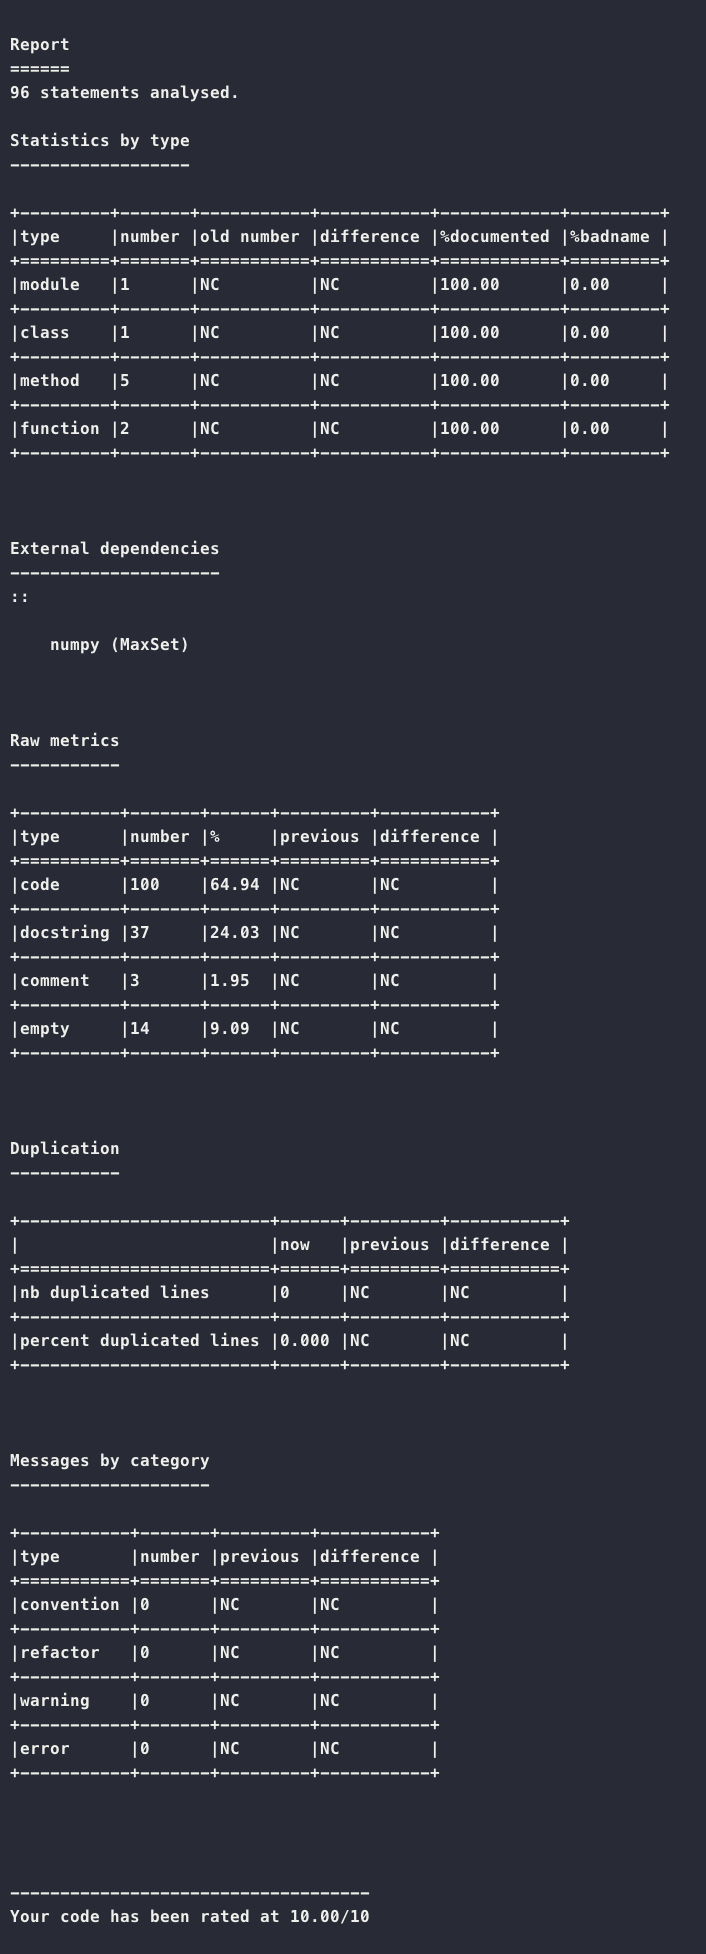
\includegraphics[scale = 0.65]{11.png}
\end{center}
\section{程序的可扩展性}
我们在基础要求实现的情况下,增加了二维数组的最大子数组求值以及一位数组的最大子数组打印功能。且对于维度很大的数组,使用list类型的元素在理论上可以对数组维度和数组长度进行无限延伸,且list类型支持多种类型的数据混用,可以实现浮点数和整数的混合数组。在未来,我们可能会实现一维数组的求值过程的可视化打印显示。
\section{两个原则}
\subsection{单一职责原则}
在本次实验设计中,MSA类专门用来来进行数据的计算,不参与程序的读入数据或处理数据类型等问题的部分,变化的原因只有需要实现的求值功能的增删改才会对这一部分进行变化;而main函数和get\_sum和get\_list函数专门对数据进行处理并进行错误处理,变化的原因只有输入数据类型的变化才会有变化,体现了单一职责原则。
\subsection{开放-封闭原则}
MSA模块的成员函数max\_list的职责是求出一位数组的最大子数组和,这一部分的内容是不必进行更改的,其他维度的最大子数组和都是依托于这一部分层层累积叠加,是可以扩展的,满足开放-封闭原则。
\section{错误处理}
该部分已经在第一部分中用\textcolor[rgb]{0,0.8,1}{蓝色字体}进行讲解,在此不再赘述。
\section{性能分析}
我们利用yappi工具对程序运行的时间进行测试,测试样例分别为$1\times 10^8$维度的整形矩阵、$1\times 10^8$维度的浮点型向量、$10^4\times 10^4$维度的整形矩阵,测试平台为macOS 12.3系统python3.7版本,其测试代码和测试结果如下:
\begin{lstlisting}[language = Python]
import yappi
import numpy as np
import MaxSet


yappi.clear_stats()
test1 = [np.random.randint(1, 1000) for i in range(100000000)]
test2 = [np.random.rand() for i in range(100000000)]
test3 = [[np.random.randint(1, 1000) for i in range(10000)] for j in range(10000)]
yappi.start()
MaxSet.get_list(test1)
yappi.stop()
stats = yappi.convert2pstats(yappi.get_func_stats())
stats.sort_stats("cumulative")
stats.print_stats()

yappi.start()
MaxSet.get_list(test2)
yappi.stop()
stats = yappi.convert2pstats(yappi.get_func_stats())
stats.sort_stats("cumulative")
stats.print_stats()

yappi.start()
MaxSet.get_list(test3)
yappi.stop()
stats = yappi.convert2pstats(yappi.get_func_stats())
stats.sort_stats("cumulative")
stats.print_stats()
\end{lstlisting}
\begin{center}
   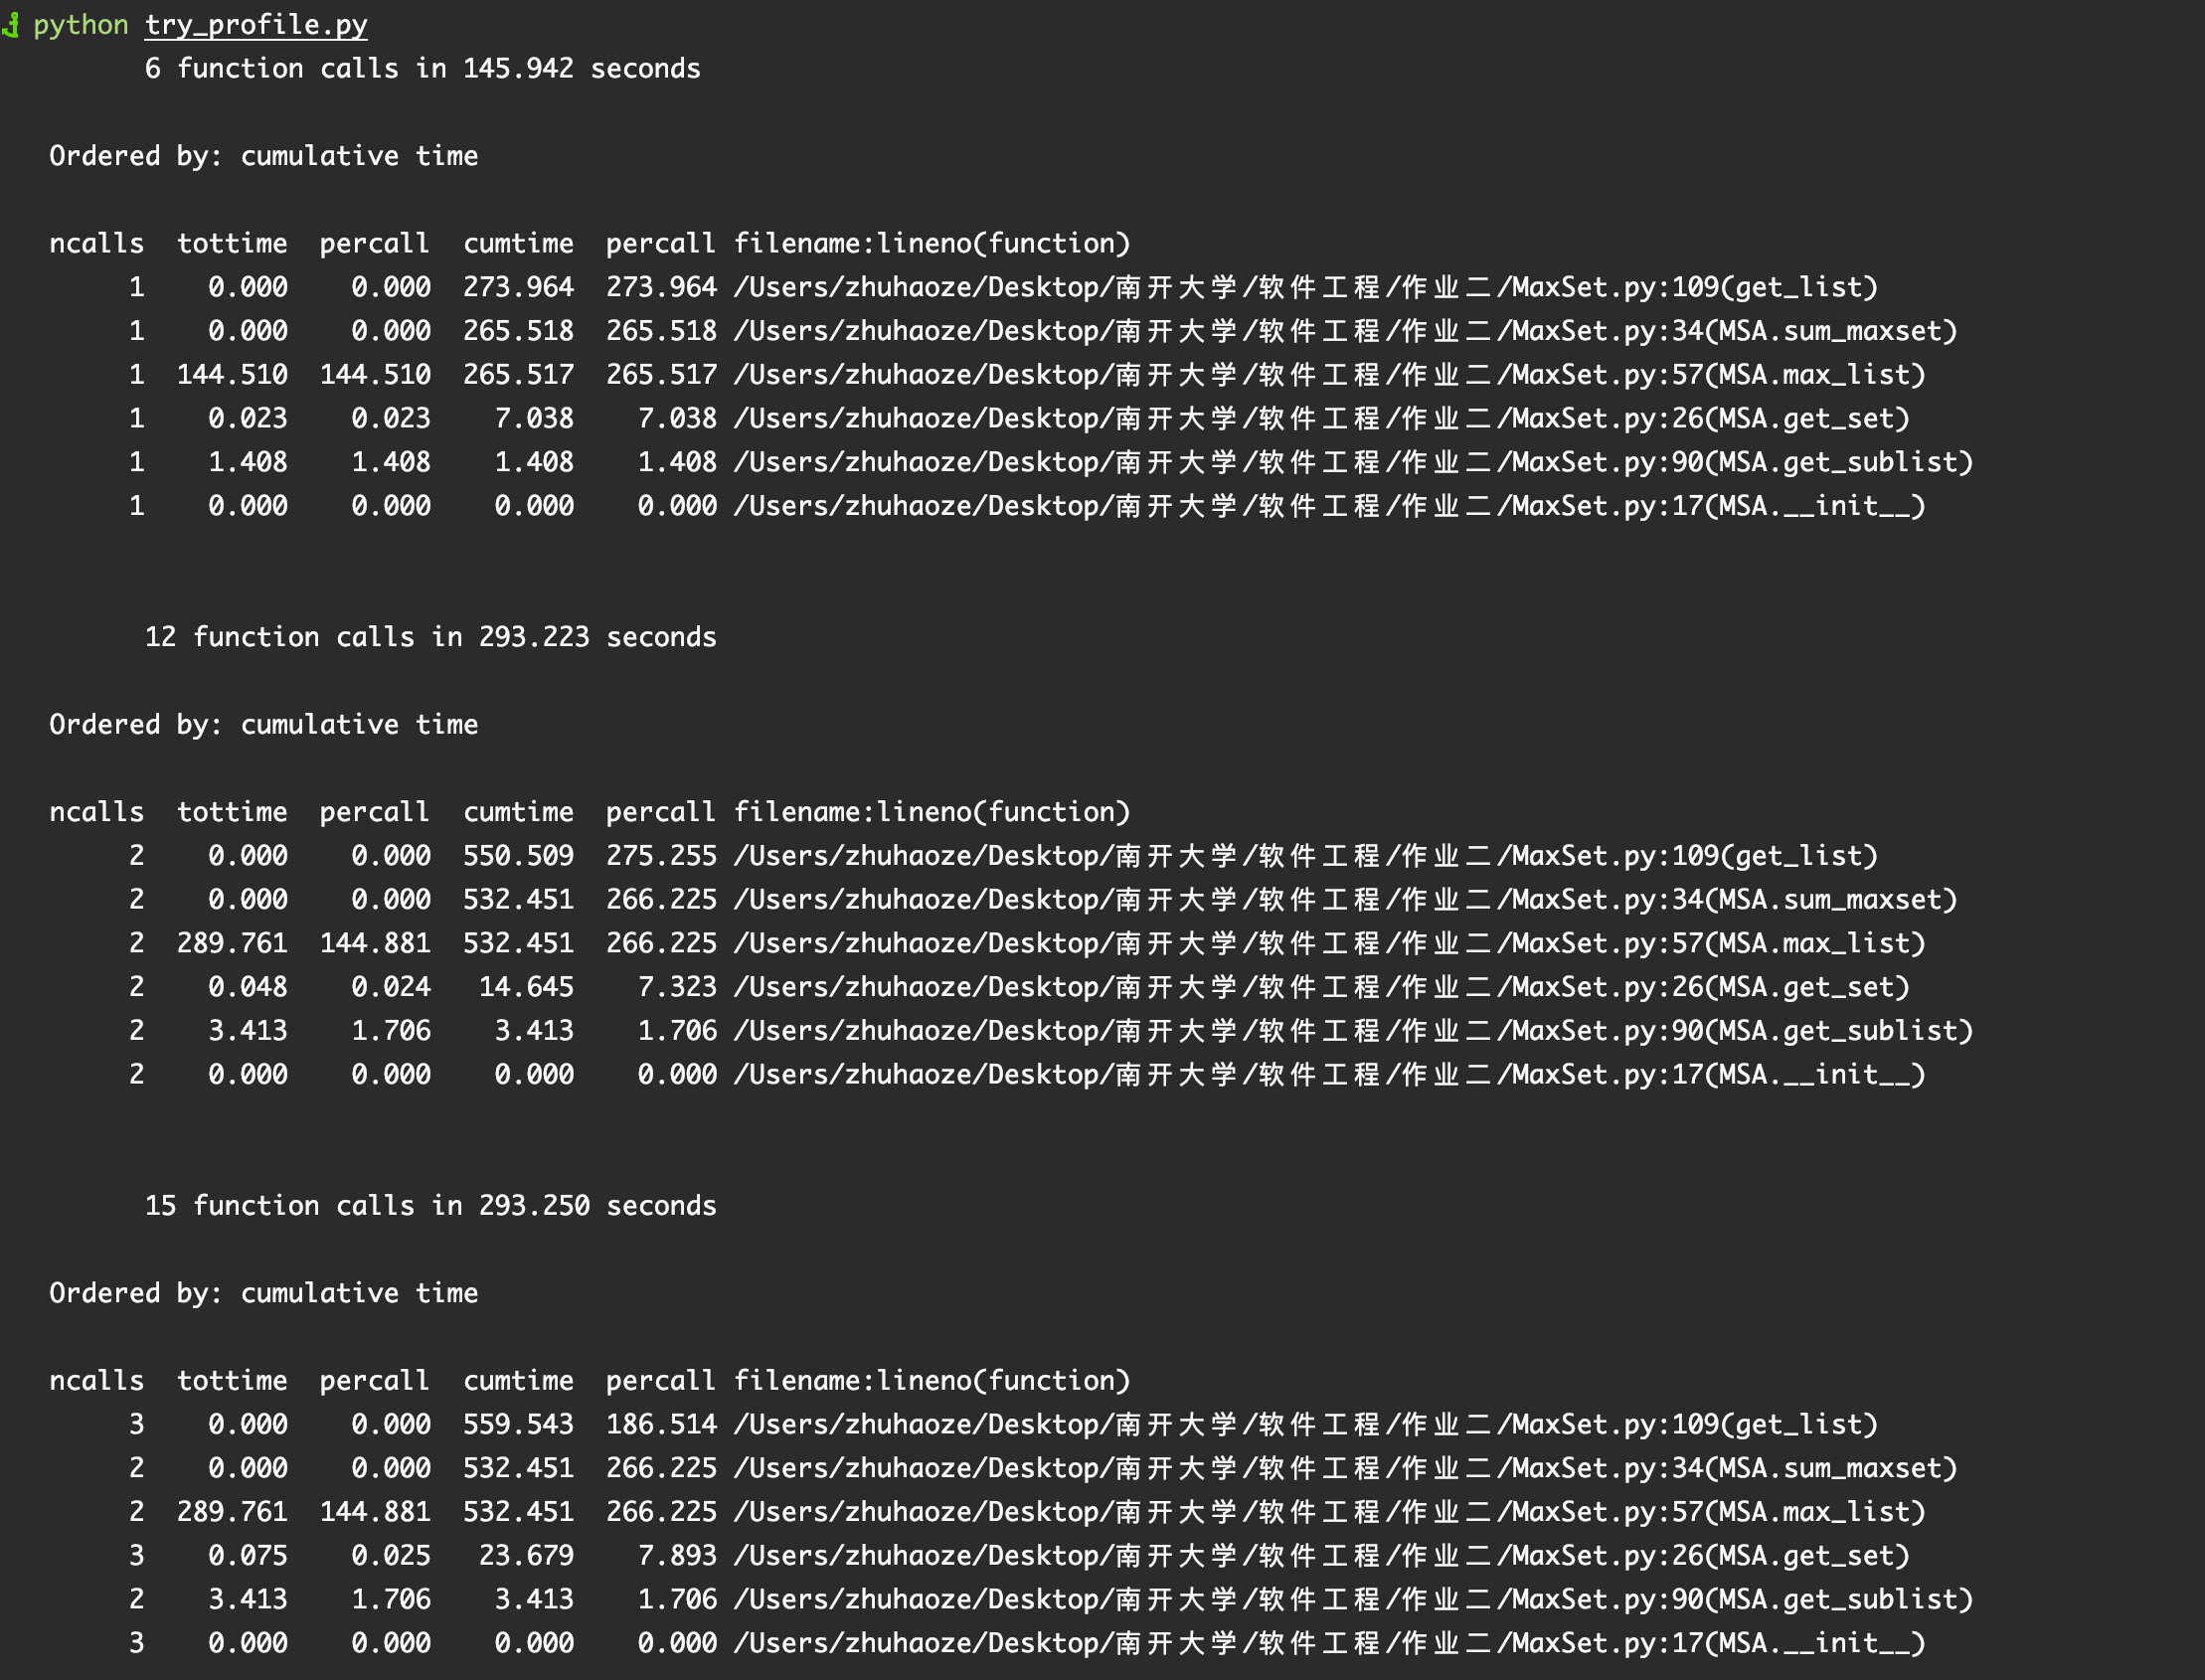
\includegraphics[scale = 0.4]{2.png}
\end{center}
\par 查看运行时间可以看出,主要时间花在了求一位数组的最大子数组这一部分,所以我们重点对这一部分进行优化。
\par 通过分析我们所写的代码可以知道,一组数组的求最大值过程是将整个一维数组进行一遍遍历,时间复杂度是$O(n)$,为线性时间。这一部分最初的想法是求出所有的子数组的和,实时更新最大值来进行求解,这样的做法的时间复杂度是$O(n^2)$,虽然对于一维数组的最大子数组的问题来说这个时间复杂度可以接受,但是在扩展到二维数组甚至多维数组的最大子数组时,这一部分计算将进行多次迭代,这一操作变得不可接受,故通过了类似于动态规划的想法对算法进行了如上的优化。
\par 关于二维数组的最大子数组这一部分,我们的思想是根据将任意连续行合并为一行便可变成了多个最大子数组的问题,通过设置一个上边界和一个下边界,将之间的行进行合并,每次合并都调用求一位最大子数组的函数进行计算,并尝试更新最大值直到边界覆盖整个数组便完成,可以看出该算法的时间复杂度为$m\times m \times 2n $即$O(n^3)$的时间复杂度,其主要问题也是多次调用一位数组的最大子数组这一子问题,所以在第一部分对这一操作已经进行了优化,获得了不错的性能。


\section{单元测试}
我们对我们的产品进行黑盒测试。首先对于数据的正负值,我们设计了全为正数(最大子数组是其本身)、全为负数(最大子数组是其负值的最大值)、以及正值负值均包含的测试样例;对于整数和浮点数,我们设计了全为整数的测试样例、全为浮点数的测试样例、整数和浮点数混合的测试样例,测试包含了可能出现的几种数据类型;于此同时,我们也进行了错误的样例的测试,比如输入的元素非要求的列表类型、列表类型中的元素非整数或浮点数(如string)、矩阵的维度为二维以上等。具体测试样例如下:
\begin{lstlisting}[language = python]
import unittest
import MaxSet


class Testing(unittest.TestCase):
   """
   测试
   """

   def test_getsum(self):
      self.assertEqual(MaxSet.get_sum([-1, 2, 3, -4]), 5)
      self.assertEqual(MaxSet.get_sum([1, 2, 3, 4]), 10)
      self.assertEqual(MaxSet.get_sum([-1, 2, -5, 3, -4]), 3)
      self.assertEqual(MaxSet.get_sum([-1, 20, -5, 30, -4]), 45)
      self.assertEqual(MaxSet.get_sum([-2, -3, -5, -1, -9]), -1)
      self.assertEqual(MaxSet.get_sum([-2.0, -3.0, -5.0, -1.0, -9.0]), -1)
      self.assertEqual(MaxSet.get_sum([-2.0, -3.0, -5.0, -1, -9]), -1)

   def test_getlist(self):
      self.assertEqual(MaxSet.get_list([-1, 2, 3, -4]), [2, 3])
      self.assertEqual(MaxSet.get_list([1, 2, 3, 4]), [1, 2, 3, 4])
      self.assertEqual(MaxSet.get_list([-1, 2, -5, 3, -4]), [3])
      self.assertEqual(MaxSet.get_list([-1, 20, -5, 30, -4]), [20, -5, 30])
      self.assertEqual(MaxSet.get_list([-1.0, 20.0, -5.0, 30.0, -4.0]), [20.0, -5.0, 30.0])
      self.assertEqual(MaxSet.get_list([-1.0, 20.0, -5, 30, -4]), [20.0, -5, 30])
      self.assertEqual(MaxSet.get_list([-2, -3, -5, -1, -9]), [-1])

   def test_sum2D(self):
      self.assertEqual(MaxSet.get_sum([[-1, -1],
                                       [-1, -1]]), -1)
      self.assertEqual(MaxSet.get_sum([[1, 1],
                                       [1, 1]]), 4)
      self.assertEqual(MaxSet.get_sum([[-15, -21, 5, -12],
                                       [-7, 21, 20, 12],
                                       [21, 0, -1, 13],
                                       [10, 20, -10, -18]]), 81)
      self.assertEqual(MaxSet.get_sum([[3, 6, 8, 9],
                                       [2, 5, 1, 8],
                                       [4, 7, 3, 9]]), 65)
      self.assertEqual(MaxSet.get_sum([[10, 1, 2, 3, 34],
                                       [1, -1, -3, -5, 98],
                                       [-8, 9, 7, -2, 2]]), 148)
      self.assertEqual(MaxSet.get_sum([[10, 1, 2, 3, 34],
                                       [1, 23, -3, -5, -34],
                                       [-8, 9, 7, -31, 2]]), 50)
      self.assertEqual(MaxSet.get_sum([[10, 1, -50, 3, 34],
                                       [-3, 25, 25, 50, -34],
                                       [-8, 9, 7, -31, -2]]), 100)
      self.assertEqual(MaxSet.get_sum([[10, 1, -50, 3, 34],
                                       [-3, 25, -25, 50, -34],
                                       [-8, 9, 7, -31, -2]]), 53)

      self.assertEqual(MaxSet.get_sum([[10.0, 1.0, -50.0, 3.0, 34.0],
                                       [-3, 25, -25, 50, -34],
                                       [-8, 9, 7, -31, -2]]), 53)

      self.assertEqual(MaxSet.get_sum([[10.0, 1.0, -50.0, 3.0, 34.0],
                                       [-3.0, 25.0, -25.0, 50.0, -34.0],
                                       [-8.0, 9.0, 7.0, -31.0, -2.0]]), 53)

   @unittest.expectedFailure
   def test_error(self):
      self.assertEqual(MaxSet.get_sum([[[10.0, 1.0, -50.0, 3.0, 34.0],
                                       [-3.0, 25.0, -25.0, 50.0, -34.0],
                                       [-8.0, 9.0, 7.0, -31.0, -2.0]], [[1]]]), 53)
      self.assertEqual(MaxSet.get_sum([[-50.0, 3.0, 34.0],
                                       [-3.0, 25.0, -25.0, 50.0, -34.0],
                                       [-8.0, 9.0, 7.0, -31.0, -2.0]]), 53)
      self.assertEqual(MaxSet.get_sum(['a', 'b', 'c']), 1)
      self.assertEqual(MaxSet.get_sum(1), 1)

\end{lstlisting}
\begin{center}
   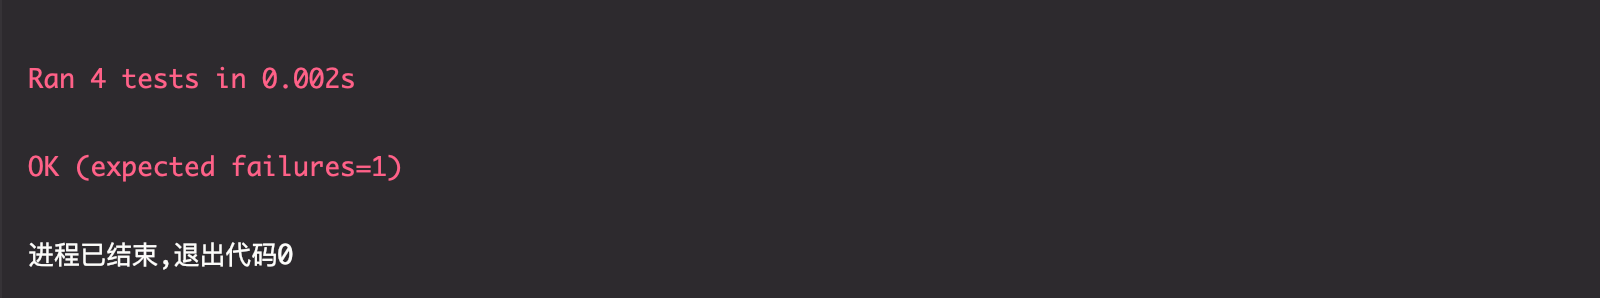
\includegraphics[scale = 0.62]{3.png}
\end{center}
由上图可见,按照条件覆盖,所有的可能条件都被考虑到,条件覆盖率为100\%,且我们的测试通过率为100\%。
\end{document}

